% Options for packages loaded elsewhere
% Options for packages loaded elsewhere
\PassOptionsToPackage{unicode}{hyperref}
\PassOptionsToPackage{hyphens}{url}
\PassOptionsToPackage{dvipsnames,svgnames,x11names}{xcolor}
%
\documentclass[
]{article}
\usepackage{xcolor}
\usepackage{amsmath,amssymb}
\setcounter{secnumdepth}{5}
\usepackage{iftex}
\ifPDFTeX
  \usepackage[T1]{fontenc}
  \usepackage[utf8]{inputenc}
  \usepackage{textcomp} % provide euro and other symbols
\else % if luatex or xetex
  \usepackage{unicode-math} % this also loads fontspec
  \defaultfontfeatures{Scale=MatchLowercase}
  \defaultfontfeatures[\rmfamily]{Ligatures=TeX,Scale=1}
\fi
\usepackage{lmodern}
\ifPDFTeX\else
  % xetex/luatex font selection
\fi
% Use upquote if available, for straight quotes in verbatim environments
\IfFileExists{upquote.sty}{\usepackage{upquote}}{}
\IfFileExists{microtype.sty}{% use microtype if available
  \usepackage[]{microtype}
  \UseMicrotypeSet[protrusion]{basicmath} % disable protrusion for tt fonts
}{}
\makeatletter
\@ifundefined{KOMAClassName}{% if non-KOMA class
  \IfFileExists{parskip.sty}{%
    \usepackage{parskip}
  }{% else
    \setlength{\parindent}{0pt}
    \setlength{\parskip}{6pt plus 2pt minus 1pt}}
}{% if KOMA class
  \KOMAoptions{parskip=half}}
\makeatother
% Make \paragraph and \subparagraph free-standing
\makeatletter
\ifx\paragraph\undefined\else
  \let\oldparagraph\paragraph
  \renewcommand{\paragraph}{
    \@ifstar
      \xxxParagraphStar
      \xxxParagraphNoStar
  }
  \newcommand{\xxxParagraphStar}[1]{\oldparagraph*{#1}\mbox{}}
  \newcommand{\xxxParagraphNoStar}[1]{\oldparagraph{#1}\mbox{}}
\fi
\ifx\subparagraph\undefined\else
  \let\oldsubparagraph\subparagraph
  \renewcommand{\subparagraph}{
    \@ifstar
      \xxxSubParagraphStar
      \xxxSubParagraphNoStar
  }
  \newcommand{\xxxSubParagraphStar}[1]{\oldsubparagraph*{#1}\mbox{}}
  \newcommand{\xxxSubParagraphNoStar}[1]{\oldsubparagraph{#1}\mbox{}}
\fi
\makeatother


\usepackage{longtable,booktabs,array}
\usepackage{calc} % for calculating minipage widths
% Correct order of tables after \paragraph or \subparagraph
\usepackage{etoolbox}
\makeatletter
\patchcmd\longtable{\par}{\if@noskipsec\mbox{}\fi\par}{}{}
\makeatother
% Allow footnotes in longtable head/foot
\IfFileExists{footnotehyper.sty}{\usepackage{footnotehyper}}{\usepackage{footnote}}
\makesavenoteenv{longtable}
\usepackage{graphicx}
\makeatletter
\newsavebox\pandoc@box
\newcommand*\pandocbounded[1]{% scales image to fit in text height/width
  \sbox\pandoc@box{#1}%
  \Gscale@div\@tempa{\textheight}{\dimexpr\ht\pandoc@box+\dp\pandoc@box\relax}%
  \Gscale@div\@tempb{\linewidth}{\wd\pandoc@box}%
  \ifdim\@tempb\p@<\@tempa\p@\let\@tempa\@tempb\fi% select the smaller of both
  \ifdim\@tempa\p@<\p@\scalebox{\@tempa}{\usebox\pandoc@box}%
  \else\usebox{\pandoc@box}%
  \fi%
}
% Set default figure placement to htbp
\def\fps@figure{htbp}
\makeatother


% definitions for citeproc citations
\NewDocumentCommand\citeproctext{}{}
\NewDocumentCommand\citeproc{mm}{%
  \begingroup\def\citeproctext{#2}\cite{#1}\endgroup}
\makeatletter
 % allow citations to break across lines
 \let\@cite@ofmt\@firstofone
 % avoid brackets around text for \cite:
 \def\@biblabel#1{}
 \def\@cite#1#2{{#1\if@tempswa , #2\fi}}
\makeatother
\newlength{\cslhangindent}
\setlength{\cslhangindent}{1.5em}
\newlength{\csllabelwidth}
\setlength{\csllabelwidth}{3em}
\newenvironment{CSLReferences}[2] % #1 hanging-indent, #2 entry-spacing
 {\begin{list}{}{%
  \setlength{\itemindent}{0pt}
  \setlength{\leftmargin}{0pt}
  \setlength{\parsep}{0pt}
  % turn on hanging indent if param 1 is 1
  \ifodd #1
   \setlength{\leftmargin}{\cslhangindent}
   \setlength{\itemindent}{-1\cslhangindent}
  \fi
  % set entry spacing
  \setlength{\itemsep}{#2\baselineskip}}}
 {\end{list}}
\usepackage{calc}
\newcommand{\CSLBlock}[1]{\hfill\break\parbox[t]{\linewidth}{\strut\ignorespaces#1\strut}}
\newcommand{\CSLLeftMargin}[1]{\parbox[t]{\csllabelwidth}{\strut#1\strut}}
\newcommand{\CSLRightInline}[1]{\parbox[t]{\linewidth - \csllabelwidth}{\strut#1\strut}}
\newcommand{\CSLIndent}[1]{\hspace{\cslhangindent}#1}



\setlength{\emergencystretch}{3em} % prevent overfull lines

\providecommand{\tightlist}{%
  \setlength{\itemsep}{0pt}\setlength{\parskip}{0pt}}



 


\makeatletter
\@ifpackageloaded{caption}{}{\usepackage{caption}}
\AtBeginDocument{%
\ifdefined\contentsname
  \renewcommand*\contentsname{Table of contents}
\else
  \newcommand\contentsname{Table of contents}
\fi
\ifdefined\listfigurename
  \renewcommand*\listfigurename{List of Figures}
\else
  \newcommand\listfigurename{List of Figures}
\fi
\ifdefined\listtablename
  \renewcommand*\listtablename{List of Tables}
\else
  \newcommand\listtablename{List of Tables}
\fi
\ifdefined\figurename
  \renewcommand*\figurename{Figure}
\else
  \newcommand\figurename{Figure}
\fi
\ifdefined\tablename
  \renewcommand*\tablename{Table}
\else
  \newcommand\tablename{Table}
\fi
}
\@ifpackageloaded{float}{}{\usepackage{float}}
\floatstyle{ruled}
\@ifundefined{c@chapter}{\newfloat{codelisting}{h}{lop}}{\newfloat{codelisting}{h}{lop}[chapter]}
\floatname{codelisting}{Listing}
\newcommand*\listoflistings{\listof{codelisting}{List of Listings}}
\makeatother
\makeatletter
\makeatother
\makeatletter
\@ifpackageloaded{caption}{}{\usepackage{caption}}
\@ifpackageloaded{subcaption}{}{\usepackage{subcaption}}
\makeatother
\usepackage{bookmark}
\IfFileExists{xurl.sty}{\usepackage{xurl}}{} % add URL line breaks if available
\urlstyle{same}
\hypersetup{
  pdftitle={Reconstructing deep-time food webs: model assumptions drive paleoecological inference},
  pdfauthor={Tanya Strydom; Baran Karapunar; Andrew P. Beckerman; Alexander Dunhill},
  pdfkeywords={food web, network construction},
  colorlinks=true,
  linkcolor={blue},
  filecolor={Maroon},
  citecolor={Blue},
  urlcolor={Blue},
  pdfcreator={LaTeX via pandoc}}



\title{Reconstructing deep-time food webs: model assumptions drive
paleoecological inference}
\author{Tanya Strydom %
%
\textsuperscript{%
%
1%
}%
; Baran Karapunar %
%
\textsuperscript{%
%
2%
}%
; Andrew P. Beckerman %
%
\textsuperscript{%
%
1%
}%
; Alexander Dunhill %
%
\textsuperscript{%
%
2%
}%
}
\date{2026-01-07}

\usepackage{setspace}
\usepackage[left]{lineno}
\usepackage[letterpaper]{geometry}

\usepackage[nolists,noheads,markers]{endfloat}
\geometry{margin=2.5cm}

\begin{document}

\thispagestyle{empty}
{\bfseries\sffamily\Large Reconstructing deep-time food webs: model
assumptions drive paleoecological inference}
\vfil
Tanya Strydom %
%
\textsuperscript{%
%
1%
}%
; Baran Karapunar %
%
\textsuperscript{%
%
2%
}%
; Andrew P. Beckerman %
%
\textsuperscript{%
%
1%
}%
; Alexander Dunhill %
%
\textsuperscript{%
%
2%
}%

\vfil
{\small
\textbf{Abstract:} Food webs provide a powerful lens for understanding
ecosystem structure and function, but reconstructing them in
paleoecological contexts remains challenging because direct evidence of
feeding interactions is rarely preserved. A wide range of models now
exist for predicting interactions and inferring network structure, yet
these models vary widely in their assumptions, mechanisms, and data
requirements. Here, we evaluate which network construction approaches
are most suitable for paleo-food-web reconstruction given the
constraints of the fossil record, and we assess how model choice shapes
the networks we infer. Using the Toarcian Oceanic Anoxic Event (Early
Jurassic, \textasciitilde183 Ma) as a case study, we compare six
modelling approaches encompassing mechanistic, structural, and
theory-based methods. These models yield strikingly different network
structures and pairwise interactions, and that these discrepancies
propagate into ecological inference, including conclusions about
extinction dynamics. Our results highlight the importance of the need to
align model choice with research questions and underscore the
interpretative risks of treating all food-web reconstruction methods as
interchangeable.
\vfil
\textbf{Keywords:} %
food web, %
network construction%
}
\clearpage
\setcounter{page}{1}
\doublespacing
\linenumbers


There has been growing interest in using deep-time fossil data to
understand how species interacted with each other in past ecosystems
(\emph{e.g.,} Dunne et al. (2008); Dunne et al. (2014)) and how
ecological communities responded to past environmental change (Dillon et
al., 2022; Kiessling et al., 2019). In modern ecosystems, species
interactions and the networks that they form have become central to
studying biodiversity, energy flow, and community stability
(\emph{e.g.,} Thuiller et al. (2024)). Network prediction tools derived
from modern ecology have increasingly been applied by paleoecologists to
reconstruct ancient food webs to gain insight into how the biosphere
responds to major environmental transitions (\emph{e.g.,} Dunhill et al.
(2024); Hao et al. (2025); Yeakel et al. (2014)). However, we are faced
by the limitation that interactions cannot be directly observed in the
fossil record (with the exception of rare instances \emph{e.g.,} Jenny
et al. (2019); Vullo (2011)) and as a result, the reconstruction of
paleo food webs depends on models that allow us to infer feeding
relationships from preserved traits, analogies to modern taxa, or
ecological theory. While numerous models exist for inferring
interactions (see Morales-Castilla et al. (2015); Pichler \& Hartig
(2023); Strydom et al. (2021); Allesina et al. (2008) for broader
reviews), only a subset can reliably be applied in paleo contexts, where
data on traits, abundances, and community composition are inherently
incomplete and biased.

The growing interest in paleo food webs has outpaced a clear discussion
of \emph{which} construction methods are suitable for which purposes.
Different models generate different kinds of networks (\emph{e.g.,}
feasible, realised, or purely structural) and these differences can
fundamentally alter ecological interpretations. In this study, we
evaluate a suite of methods that can be feasibly applied to paleo
communities and explore how their underlying assumptions shape both
network structure and ecological inference. Specifically we focus on
identifying a suite of models that are appropriate for use with paleo
data that can feasibly be constructed within the limitations that are
imposed by fossil data while still intersecting across the different
network types. Here we use the data from Dunhill et al. (2024) to
reconstruct communities across the Toarcian extinction event using a
suite of different modelling approaches. We ask (i) how do different
models vary in the network structures and pairwise interactions they
recover, and (ii) to what extent does model choice influence ecological
inference, including which factors are interpreted as the dominant
drivers of extinction across a major extinction event..

\section{Constructing paleo webs}\label{constructing-paleo-webs}

\subsection{Challenges specific to building paleo
networks}\label{challenges-specific-to-building-paleo-networks}

Reconstructing paleo food webs presents challenges that differ from
those encountered in modern systems. First, the fossil record provides
an incomplete and selectively preserved subset of the original
community. Preservation biases (driven by habitat, skeletal composition,
and sedimentary environment) mean that some trophic groups are
over-represented (e.g., hard-shelled organisms), while others (e.g.,
soft-bodied taxa, plankton) are systematically under-sampled. This
directly constrains the kinds of models that can be applied, because
models requiring complete assemblages or accurate guild representation
will perform poorly when preservation is uneven \textbf{(REF)}.
Furthermore, there is inherent uncertainty about the true community
compositions. Fossil assemblages may represent time-averaged ``death
assemblage'' accumulations, transported material, or mixed habitats,
rather than true representations of ``life assemblages'' of organisms
that interacted with one another. As a result, any paleontological
assemblage is best interpreted as a set of taxa that could have
interacted, rather than a snapshot of a specific subset of interacting
organisms. Moreover, certain traits cannot be reliably estimated, such
as body size due to disarticulation (e.g., echinoderms) or partial
preservation (e.g., sharks), or species abundances due to
time-averaging, transportation, or preservation. These shortcomings
limit the potential models that can be applied to reconstruct trophic
networks from fossil assemblages. Additionally, many extinct taxa have
ambiguous trait states, especially regarding diet and behaviour. Even
when functional morphology is preserved, ecological behaviour is seldom
directly evident. Such uncertainty propagates differently across model
families: mechanistic models \textbf{(e.g., xxx, Figure 1)} tend to
accommodate broad trait assignments, whereas theory-driven models
\textbf{(e.g., xxx)} are more sensitive to uncertainty in body size,
foraging mode, or feeding constraints. These limitations do not render
reconstruction impossible but highlight the importance of choosing a
model whose assumptions match the type of ecological inference being
attempted.

\subsection{Understanding the approaches to network
construction}\label{understanding-the-approaches-to-network-construction}

Network construction approaches can be broadly grouped into three
methodological and conceptual approaches Figure~\ref{fig-concept}. The
first are mechanistic models which evaluate whether an interaction is
\emph{feasibly possible}. These models typically use trait-based rules
(\emph{e.g.,} feeding mode, body size, or functional morphology) or
evolutionary relationships to determine whether a species \emph{could}
consume another, by extension this also allows us to identify forbidden
links (\emph{i.e.,} interactions that are mechanistically incompatible
Jordano (2016)). Mechanistic approaches tend to produce metawebs - the
full set of all plausible interactions given biological constraints.
Theory-driven models embed assumptions from ecological theory (such as
niche theory or foraging ecology) to generate realised interactions and
networks. Structural models are similar to theory-driven models, with
the exception that these models are species agnostic and as such can
only be used to make inferences about network structure \textbf{(i.e.,
xxx)} rather than inferring realistic pairwise predator-prey links. Both
theory-driven and structural models aim to reproduce characteristic
patterns observed in modern food webs, such as intervality, trophic
hierarchies, or body-size-scaled feeding ranges. They do not necessarily
require detailed trait information and instead rely on ecological rules
or statistical distributions consistent with empirical food webs.

\begin{figure}

\centering{

\pandocbounded{\includegraphics[keepaspectratio]{figures/model_fams.png}}

}

\caption{\label{fig-concept}This obviously needs work but a variation on
this to try and articulate the different approaches and broadly how they
may differ.}

\end{figure}%

Most existing paleo-specific approaches fall within the mechanistic
space (e.g., Shaw et al. (2024); Roopnarine (2006); Fricke et al.
(2022)). While these are well-suited for reconstructing feasible
interactions, they represent only a subset of the broader space of
network construction methods. Incorporating theory-driven models allows
paleoecologists to explore realised interaction structures and address a
wider suite of ecological questions---provided their assumptions are
compatible with the limitations of fossil data. Here we present a range
of models Table~\ref{tbl-models} that carry specific assumptions and
data requirements. For instance, allometric models depend on
quantitative body-size estimates, which must be inferred from size
classes or functional morphology in the fossil record. Structural models
such as the niche model require only richness and connectance, but their
species-agnostic nature limits their usefulness for trait-based or
diet-specific questions. Mechanistic models rely on accurate assignment
of feeding traits, which may be uncertain for extinct taxa but are often
more tractable than estimating abundances or interaction strengths.
Understanding how these limitations intersect with what fossil data can
reliably provide is essential for selecting an appropriate modelling
approach.

\begin{longtable}[]{@{}
  >{\raggedright\arraybackslash}p{(\linewidth - 10\tabcolsep) * \real{0.1667}}
  >{\raggedright\arraybackslash}p{(\linewidth - 10\tabcolsep) * \real{0.1667}}
  >{\raggedright\arraybackslash}p{(\linewidth - 10\tabcolsep) * \real{0.1667}}
  >{\raggedright\arraybackslash}p{(\linewidth - 10\tabcolsep) * \real{0.1667}}
  >{\raggedright\arraybackslash}p{(\linewidth - 10\tabcolsep) * \real{0.1667}}
  >{\raggedright\arraybackslash}p{(\linewidth - 10\tabcolsep) * \real{0.1667}}@{}}
\caption{Six different models that can be used to construct food webs
for both this specific community but are also broadly suited to paleo
network prediction. These models span all facets of the network
representation space (metaweb, realised, and structural network) and are
suitable for an array of different paleo communities as the data
requirements fall within the limitations set by the fossil
record.}\label{tbl-models}\tabularnewline
\toprule\noalign{}
\begin{minipage}[b]{\linewidth}\raggedright
Model family
\end{minipage} & \begin{minipage}[b]{\linewidth}\raggedright
Assumptions
\end{minipage} & \begin{minipage}[b]{\linewidth}\raggedright
Data needs
\end{minipage} & \begin{minipage}[b]{\linewidth}\raggedright
`Limitation'
\end{minipage} & \begin{minipage}[b]{\linewidth}\raggedright
Network type
\end{minipage} & \begin{minipage}[b]{\linewidth}\raggedright
Key reference
\end{minipage} \\
\midrule\noalign{}
\endfirsthead
\toprule\noalign{}
\begin{minipage}[b]{\linewidth}\raggedright
Model family
\end{minipage} & \begin{minipage}[b]{\linewidth}\raggedright
Assumptions
\end{minipage} & \begin{minipage}[b]{\linewidth}\raggedright
Data needs
\end{minipage} & \begin{minipage}[b]{\linewidth}\raggedright
`Limitation'
\end{minipage} & \begin{minipage}[b]{\linewidth}\raggedright
Network type
\end{minipage} & \begin{minipage}[b]{\linewidth}\raggedright
Key reference
\end{minipage} \\
\midrule\noalign{}
\endhead
\bottomrule\noalign{}
\endlastfoot
random & Links are randomly distributed within a network & richness,
number of links & parameter assumptions, species agnostic & structural
network & Erdős \& Rényi (1959) \\
niche & Networks are interval, species can be ordered on a `niche axis'
& richness, connectance & parameter assumptions, species agnostic &
structural network & Williams \& Martinez (2008) \\
allometric diet breadth model (ADBM) & Interactions are determined by
energetic costs (foraging ecology) & body mass, biomass (abundance) &
does not account for forbidden links in terms of trait compatibility,
assumptions on body size and biomass (abundance) from fossil data &
theoretical network & Petchey et al. (2008) \\
l-matrix & Interactions inferred using allometric rules (ratio of body
sizes between predator and prey), with links being constrained by a
Ricker function & body mass, number of producer species & does not
account for forbidden links in terms of trait compatibility, assumptions
on body size from fossil data, assumptions as to the number of producer
species & theoretical network & Schneider et al. (2016) \\
paleo food web inference model (PFIM) & Interactions can be inferred by
a mechanistic framework/relationships & feeding traits for taxa,
mechanistic feeding rules & Assumption made as to the feeding
mechanisms, need to elucidate traits from models (although this is a way
smaller issue) & mechanistic web & Shaw et al. (2024) \\
body size ratio model & Interactions inferred using allometric rules
(ratio of body sizes between predator and prey). Logit of the linking
probability used to further constrain links to an `optimal size range'
for prey. & body mass & does not account for forbidden links in terms of
evolutionary compatibility, assumptions on body size from fossil data &
theoretical network & Rohr et al. (2010) \\
\end{longtable}

\section{Case study: Toarcian mass extinction
event}\label{case-study-toarcian-mass-extinction-event}

\subsection{Dataset overview}\label{dataset-overview}

\subsubsection{Species occurrence}\label{species-occurrence}

We used fossil occurrence data spanning the upper Pliensbachian
(\textasciitilde185 Ma) to the upper Toarcian (\textasciitilde175 Ma) of
the Cleveland Basin, following Dunhill et al. (2024). The dataset
comprises four paleo-communities representing the pre-extinction,
post-extinction, early recovery, and late recovery intervals of the
Toarcian Oceanic Anoxic Event. Each assemblage was treated as a
community of potentially interacting taxa.

\subsubsection{Defining modes of life
(traits)}\label{defining-modes-of-life-traits}

We used the modes of life (traits) as identified in Dunhill et al.
(2024), who defined four traits: motility (fast, slow, facultative,
non-motile), tiering (pelagic, erect, surficial, semi-infaunal, shallow
infaunal, deep infaunal), feeding (predator, suspension feeder, deposit
feeder, mining, grazer), and size: gigantic (\textgreater500 mm), very
large (\textgreater300--500 mm), large (\textgreater100--300 mm), medium
(\textgreater50--100 mm), small (\textgreater10--50 mm), tiny (≤10 mm),
for each fossil taxon based on the ecological traits defined in the
Bambach ecospace model (Bambach et al., 2007).

\subsubsection{Constructing networks}\label{constructing-networks}

For each paleo community, we constructed 100 networks using each of the
models listed in Table~\ref{tbl-models} (6 models × 4 time intervals ×
100 replicates = 2,400 networks). Networks were then simplified by
removing disconnected species thus ensuring that all nodes participated
in at least one interaction. Models requiring body-size inputs (ADBM,
l-matrix, and body-size ratio models) were parameterised by drawing body
masses from uniform distributions bounded by the size-class limits
assigned in Dunhill et al. (2024). This approach propagates uncertainty
inherent in fossil size estimates while preserving consistent relative
sizes among species within a replicate. For each replicate, the same set
of body masses was used across models that depend on size. For
structural models (random and niche), connectance was drawn uniformly
from 0.07--0.34 to ensure networks spanned a realistic range of
empirical food-web connectances, while holding richness constant. The
same connectance value was used for both models within a replicate to
facilitate direct comparison. For each network, we calculated the
metrics listed in Table~\ref{tbl-properties}, capturing macro-, meso-,
and micro-scale structural properties.

\subsection{Models capture different network structure but in unexpected
ways}\label{models-capture-different-network-structure-but-in-unexpected-ways}

When quantifying network structure, we are essentially asking how
interactions are distributed across taxa and how these patterns scale
from individual nodes to the whole community. Structural metrics are
informative because they reflect underlying ecological processes: how
energy flows through trophic levels, how disturbances propagate, where
redundancy or fragility exists, and how species specialise or generalise
in their diets. To capture these different facets, we evaluated a suite
of macro-, meso-, and micro-scale metrics Table~\ref{tbl-properties},
ranging from global properties like connectance and complexity to motifs
and species-level generality and vulnerability.

\begin{longtable}[]{@{}
  >{\raggedright\arraybackslash}p{(\linewidth - 6\tabcolsep) * \real{0.2466}}
  >{\raggedright\arraybackslash}p{(\linewidth - 6\tabcolsep) * \real{0.2603}}
  >{\raggedright\arraybackslash}p{(\linewidth - 6\tabcolsep) * \real{0.2466}}
  >{\raggedright\arraybackslash}p{(\linewidth - 6\tabcolsep) * \real{0.2466}}@{}}
\caption{Network properties used for
analysis.}\label{tbl-properties}\tabularnewline
\toprule\noalign{}
\begin{minipage}[b]{\linewidth}\raggedright
Metric
\end{minipage} & \begin{minipage}[b]{\linewidth}\raggedright
Definition
\end{minipage} & \begin{minipage}[b]{\linewidth}\raggedright
Scale
\end{minipage} & \begin{minipage}[b]{\linewidth}\raggedright
Reference (for maths), can make footnotes probs
\end{minipage} \\
\midrule\noalign{}
\endfirsthead
\toprule\noalign{}
\begin{minipage}[b]{\linewidth}\raggedright
Metric
\end{minipage} & \begin{minipage}[b]{\linewidth}\raggedright
Definition
\end{minipage} & \begin{minipage}[b]{\linewidth}\raggedright
Scale
\end{minipage} & \begin{minipage}[b]{\linewidth}\raggedright
Reference (for maths), can make footnotes probs
\end{minipage} \\
\midrule\noalign{}
\endhead
\bottomrule\noalign{}
\endlastfoot
Richness & Number of nodes in the network & Macro & \\
Links & Normalized standard deviation of links (number of consumers plus
resources per taxon) & Micro & \\
Connectance & \(L/S^2\), where \(S\) is the number of species and \(L\)
the number of links & Macro & \\
Max trophic level & Prey-weighted trophic level averaged across taxa &
Macro & Williams \& Martinez (2004) \\
Diameter & Diameter can also be measured as the average of the distances
between each pair of nodes in the network & Macro & Delmas et al.
(2018) \\
Complexity & SVD complexity of a network, defined as the Pielou entropy
of its singular values & Macro & Strydom et al. (2021) \\
Redundancy & \((L - (S - 1))/S\), where \(S\) is the number of species
and \(L\) the number of links. Indicates the number of edges beyond what
is needed for a minimum-connected tree & Macro & \\
S1 & Number of linear chains, normalised & Meso & Milo et al. (2002);
Stouffer et al. (2007) \\
S2 & Number of omnivory motifs, normalised & Meso & Milo et al. (2002);
Stouffer et al. (2007) \\
S4 & Number of apparent competition motifs, normalised & Meso & Milo et
al. (2002); Stouffer et al. (2007) \\
S5 & Number of direct competition motifs, normalised & Meso & Milo et
al. (2002); Stouffer et al. (2007) \\
Generality & Normalized standard deviation of generality of a species
standardized by \(L/S\) & Micro & Williams \& Martinez (2000) \\
Vulnerability & Normalized standard deviation of vulnerability of a
species standardized by \(L/S\) & Micro & Williams \& Martinez (2000) \\
\end{longtable}

Despite being supplied with the same taxon pools, the different models
generated networks with systematically different structural signatures.
A MANOVA (using the metrics listed in Table~\ref{tbl-properties} as the
dependent variables and model as the grouping variable) revealed a
strong multivariate effect of model type on network structure (Pillai's
Trace = 3.89, p \textless{} 0.001), indicating that each modelling
approach produces a distinct `structural fingerprint'. Follow-up ANOVAs
confirmed that model choice had substantial effects on every metric we
examined, with effect sizes typically exceeding 0.80. The only exception
was maximum trophic level (η² = 0.19), suggesting some convergence in
vertical structure even when structure differs widely.

Post-hoc comparisons revealed three broad clusters
Figure~\ref{fig-marginal}. PFIM consistently yielded the most connected,
dense networks, reflecting its mechanistic emphasis on trait-based
feasibility. Niche, random, and body-size ratio models formed an
intermediate group, producing networks with moderate connectance and
motif frequencies. ADBM and l-matrix formed a tight cluster
characterised by constrained feeding ranges, reflecting their shared
basis in energetic and allometric theory. Although these groupings
broadly align with \emph{a priori} expectations about model families,
several patterns emerged that were less intuitive. Most notably, the
body-size ratio model, which is theoretically grounded but, aligned more
closely with structural models than with the fully theoretic ones. This
suggests that even slight differences in how body-size constraints are
implemented can shift a model's position within the network-structure
landscape. A Linear Discriminant Analysis (LDA) further illustrated the
distinctiveness of the model families Figure~\ref{fig-structure}.
Classification accuracy of the LDA was 85\%, demonstrating that the
combination of dependent variables effectively discriminates among model
types, indicating the strong imprint that model assumptions leave on
inferred ecological patterns. The PFIM model is strongly separated,
while ADBM and l-matrix networks cluster closely together. The niche and
random models occupy intermediate positions. Importantly these results
indicate that model choice is the dominant driver of inferred network
structure, often overwhelming the ecological signal embedded within the
taxon pool itself. Models designed to reproduce feasible interactions
and those designed to generate realised niche structure occupy
fundamentally different portions of `network space', even when operating
on identical taxa. Such structural divergences could have direct
implications for ecological inference, particularly when comparing
networks across time or when using network metrics to infer processes
such as community stability, trophic organisation, or susceptibility to
cascading extinctions.

\begin{figure}

\centering{

\pandocbounded{\includegraphics[keepaspectratio]{figures/marginal_mean.png}}

}

\caption{\label{fig-marginal}Estimated marginal means (EMMs) of
ecological network metrics across six model types with 95\% confidence
intervals. Bars represent the predicted values for each model, and error
bars indicate the 95\% confidence limits. Letters above each bar denote
Tukey-adjusted pairwise significance: models sharing the same letter are
not significantly different, while models with different letters are
significantly different (p \textless{} 0.05). The plot reveals three
tiers of model performance, with pfim consistently higher, log ratio,
niche, and random at intermediate levels, and adbm and l-matrix lower,
consistent with the MANOVA and post-hoc analyses.}

\end{figure}%

\begin{figure}

\centering{

\pandocbounded{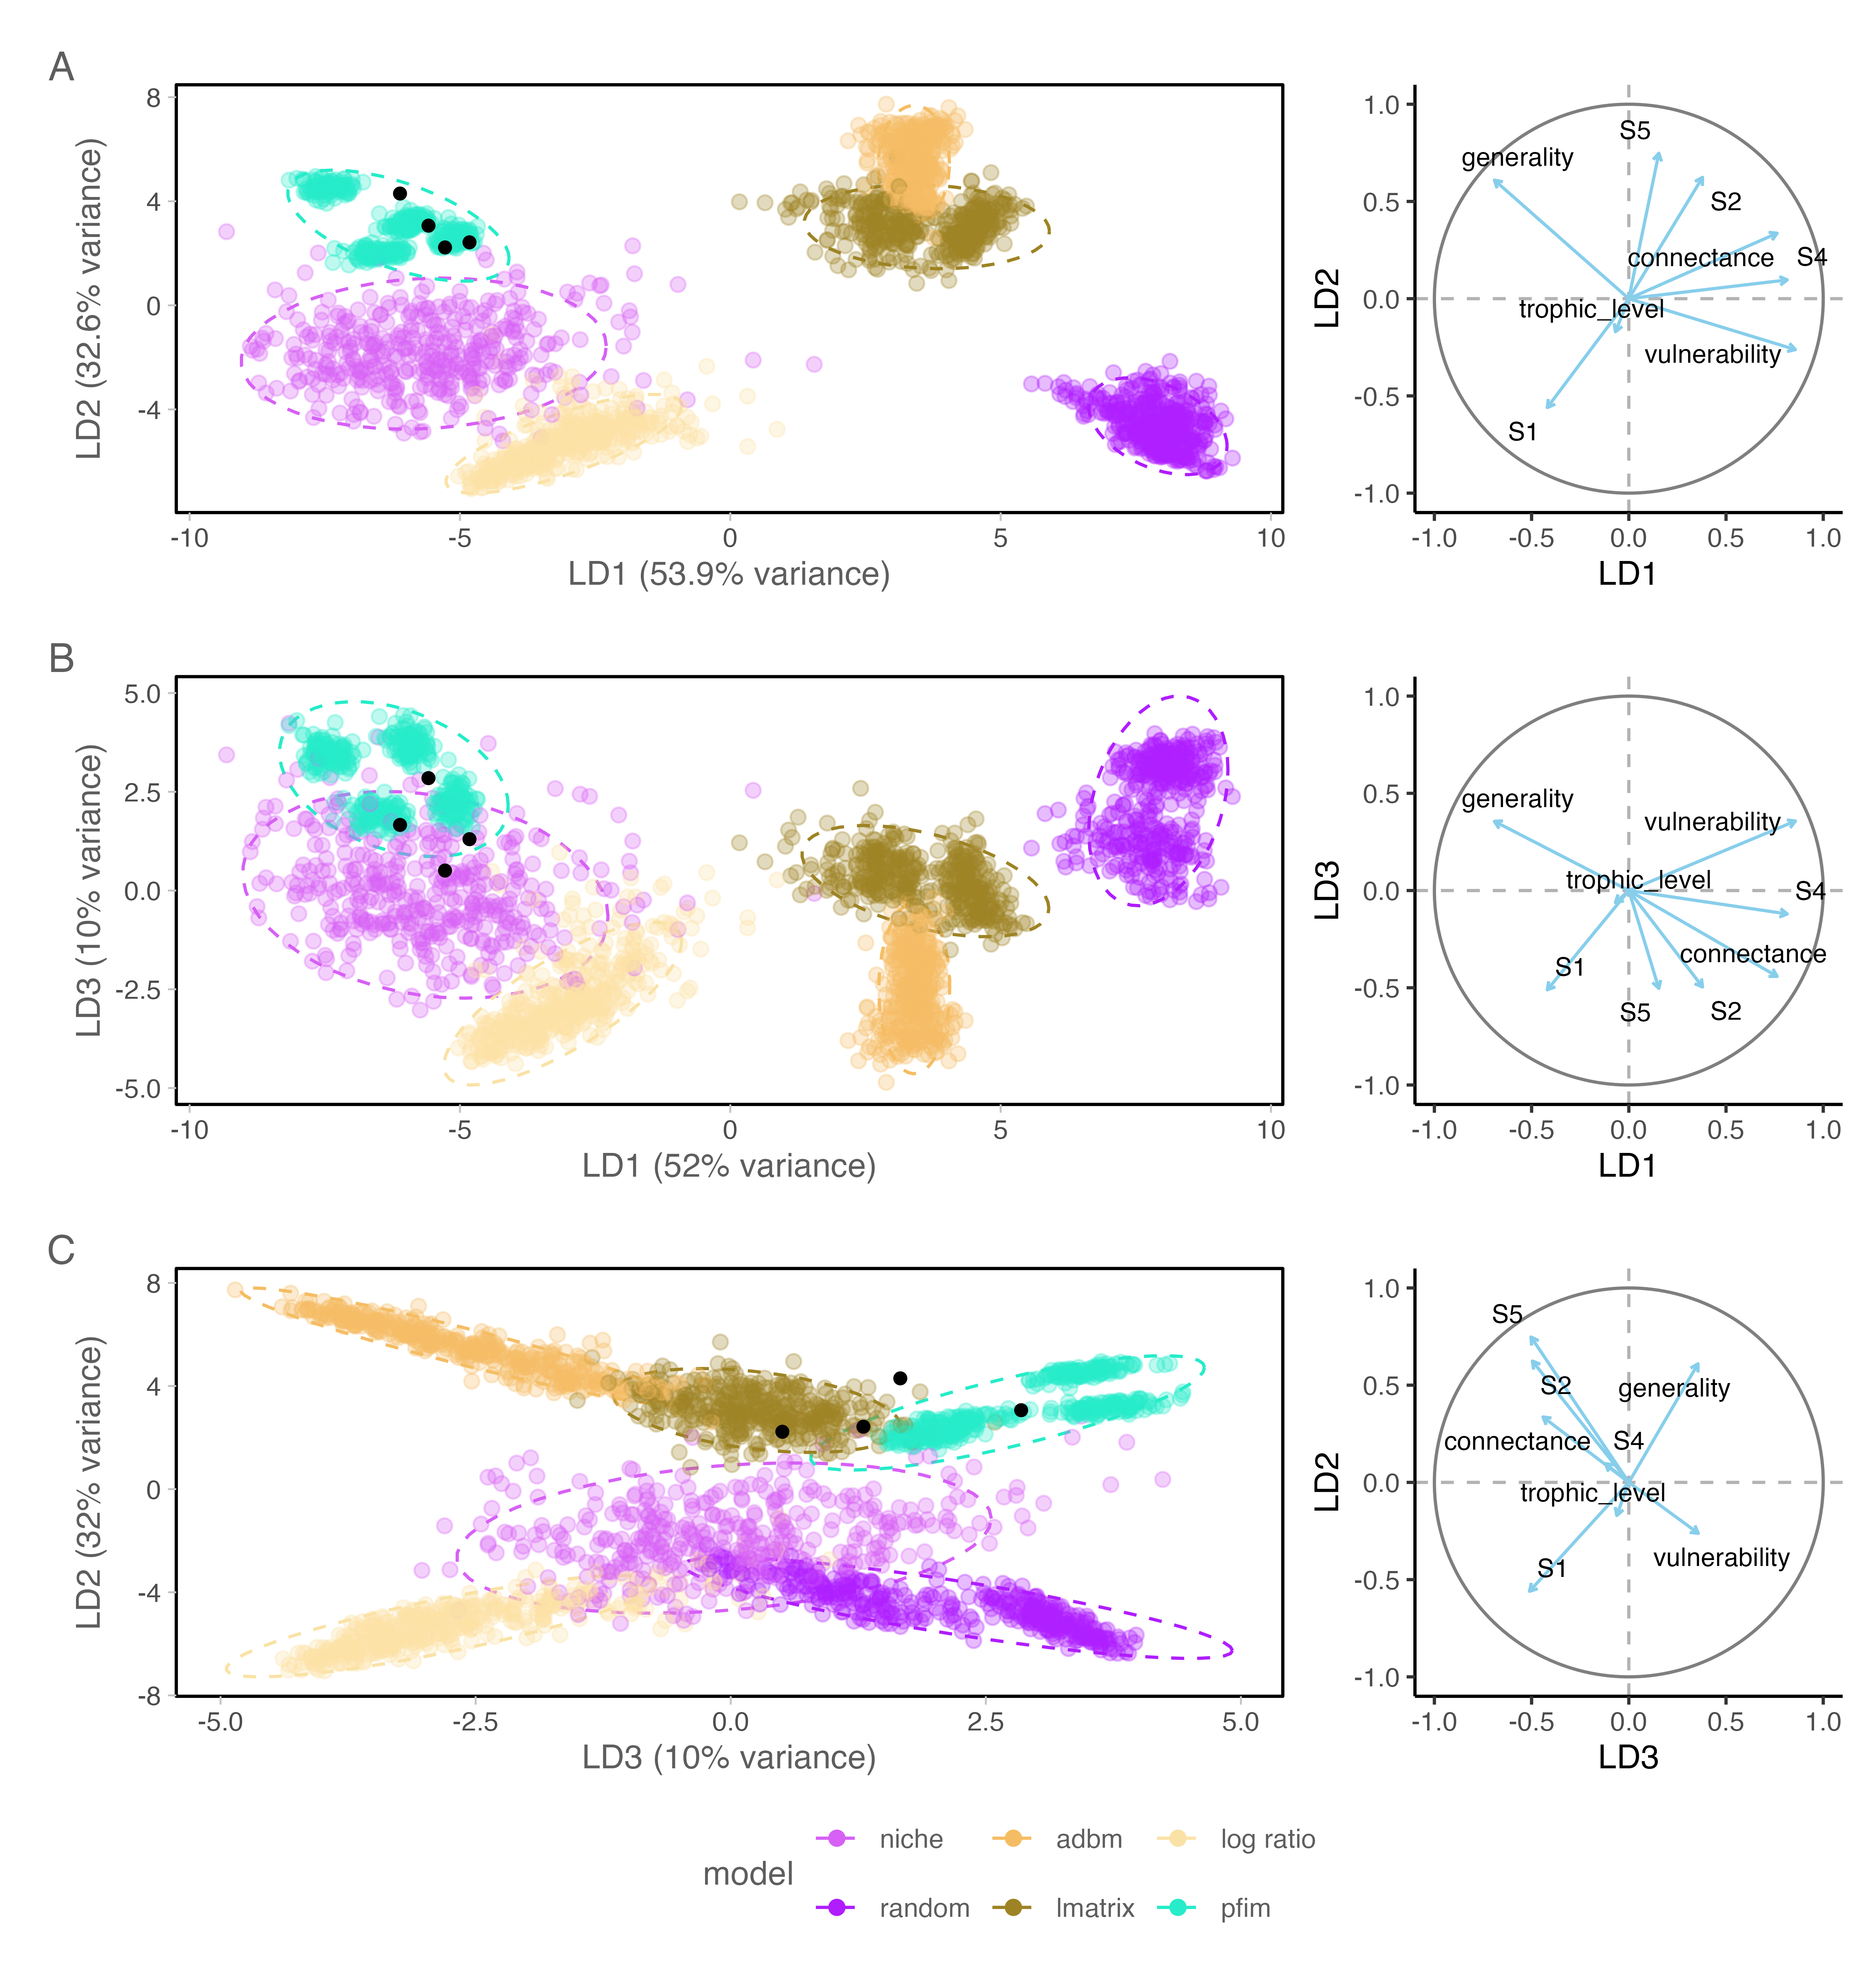
\includegraphics[keepaspectratio]{figures/MANOVA_3_panel.png}}

}

\caption{\label{fig-structure}Linear discriminant analysis (LDA) of
ecological network metrics for six model types. Each point represents a
replicate, and ellipses indicate 95\% confidence regions for each model.
The second column represents the correlation of the various network
metrics with the respective LDA axes.}

\end{figure}%

\subsection{Some networks don't share any interactions and some share a
lot}\label{some-networks-dont-share-any-interactions-and-some-share-a-lot}

Beyond differences in global structure, researchers are often interested
in~specific ecological relationships, \emph{e.g.,} who eats who, which
species share predators, and how trophic roles change across communities
or time. For these types of questions, it is essential to understand how
models differ at the level of pairwise interactions. To quantify this,
we measured interaction turnover between networks to allow us to assess
the degree to which two models predict the same or different links for
the same set of species (see Poisot et al., 2012 for methods). This is
analogous to β-diversity but applied to links rather than species.
Specifically we only looked at the dissimilarity of interaction between
shared species. Even when supplied with identical species pools, models
varied dramatically in the interactions they inferred
Figure~\ref{fig-beta_div}. Some pairs of models showed substantial
agreement, whereas others shared almost no interactions at all. Note
here that we did not include the Random or Niche models as these
networks are species agnostic and as such are not designed for inferring
species-specific pairwise links.

The body-size ratio model had consistently~high~turnover relative to all
others, indicating that it inferred diets that were largely distinct.
This reflects the strong constraints imposed by its logit-based linking
rule, which sharply restricts prey to a narrow `optimal' size range.
Small differences in body-size estimates or functional groupings
therefore lead to disproportionately large changes in inferred
interactions. In contrast, the ADBM and L-matrix showed low turnover
between each other, reflecting their shared theoretical foundations
(operationalising foraging decisions and energetic constraints using
similar allometric principles). As a result, they tend to produce
similar pairwise interactions even when implemented independently. The
PFIM exhibited intermediate turnover, sharing more interactions with
size-based theoretical models than with the body-size ratio model. This
makes sense: although PFIM uses categorical traits and hierarchical
feeding rules rather than quantitative foraging theory, these
constraints will still produce broadly similar trophic groupings.

Taken together, these patterns show that~pairwise interactions differ
far more across models than global metrics alone might suggest. Two
models with superficially similar connectance or trophic structure may
nonetheless infer completely different diets for individual taxa. This
has significant implications for any question focused on species-level
ecology, including predator--prey specialisation, trophic niche breadth,
or the identity of keystone consumers. These findings reinforce the
importance of selecting a model whose assumptions align with the
intended inference. If the goal is to explore the full set of possible
interactions a species could have had, a mechanistic model such as PFIM
is appropriate. If instead the goal is to infer the likely realised
interactions or energy pathways, models grounded in allometric foraging
theory (ADBM, L-matrix) will provide more ecologically coherent results.
Conversely, models like the body-size ratio may be too restrictive or
idiosyncratic for diet-based questions because they force interactions
into narrow, trait-determined windows.

\begin{figure}

\centering{

\pandocbounded{\includegraphics[keepaspectratio]{figures/beta_div.png}}

}

\caption{\label{fig-beta_div}Pairwise beta turnover in species
interactions among four ecological network models (adbm, lmatrix,
log-ratio, and pfim). Each cell represents the mean turnover value
between a pair of models, with warmer colors indicating greater
dissimilarity in inferred interactions. The diagonal is omitted. High
turnover values (yellow) indicate strong disagreement in network
structure between models, whereas lower values (blue--purple) indicate
greater similarity.}

\end{figure}%

\subsection{Model choice changes the
narrative}\label{model-choice-changes-the-narrative}

The structural and interaction-level differences documented above raise
a central question: do different models also lead to different
interpretations of extinction selectivity inference? In other words,
does model choice merely affect the architecture of the reconstructed
networks, or does it shape the actual stories we tell about how
communities collapsed and recovered during the Toarcian extinction
event? Using the pre-extinction networks as starting points, we
simulated species losses under a suite of ecologically plausible
extinction scenarios, including trait-based removals (e.g., body size,
motility), network-position removals (e.g., vulnerability, generality),
and random extinctions. In each case, we allowed for cascading secondary
extinctions. For each model and scenario, we then measured how closely
the simulated post-extinction network resembled the real fossil
community.

\subsubsection{Inferred extinction
drivers}\label{inferred-extinction-drivers}

To assess the consistency with which different modelling approaches
evaluate extinction scenarios, we quantified the agreement in scenario
rankings produced by each model across several network metrics. For each
model, each extinction scenario, and each network metric, we calculated
the mean absolute difference (MAD) between the observed metric value and
the value predicted following the simulated extinction sequence. Lower
MAD values indicate a closer match to the empirical network structure
and, therefore, a better-performing extinction scenario for that model
and metric. Additionally, we used a modification of Gupta et al. (2022)
true skill statistic (TSS, see Equation~\ref{eq-1}), where a score below
zero indicates that the simulated extinction performs no better than
random, and a score of one indicates a perfect match between real and
simulated. Here we calculated both a node-level TSS as well as
link-level TSS, by parsing out the TSS into two components we are able
to assess if differences between real and simulated networks are due to
node-level (the wrong taxon being removed) or link-level (the wrong
links be recovered) mismatches. Because the extinction simulations do
not allow for the origination of taxa, when calculating the TSS we only
retained taxa that were present in both the pre and post extinction
community and so any node-level mismatches between real and simulated
networks was due to the wrong taxon being removed and not because new
taxa were not.

\begin{equation}\phantomsection\label{eq-1}{ 
TSS = \frac{True Positive}{True Positive + False Negative} + \frac{True Negative}{True Negative + False Positive} - 1 
}\end{equation}

For each network metric, we treated each model as an independent
evaluator of scenario performance. MAD and TSS values were converted to
within-model rankings, with rank 1 assigned to the scenario with the
smallest MAD (\emph{i.e.,} the closest match to the empirical value) or
highest TSS score. Ranking was performed independently for each
combination of model and network metric to avoid assumptions about
comparability across metrics. To evaluate whether different models
produced consistent rankings of extinction scenarios, we quantified rank
correlation among models separately for each network metric. Agreement
among model rankings was assessed using Kendall's rank correlation
coefficient (Kendall's τ), which measures the degree of agreement
between two ordinal rankings. Kendall's τ was selected because it is
robust for small sample sizes, handles tied ranks appropriately, and
provides a direct measure of the probability that model pairs agree or
disagree on the relative ordering of scenarios. Kendall's τ ranges from
--1 to +1, where +1 indicates perfect agreement between rankings, 0
reflects no relationship, and --1 represents complete disagreement such
that one ranking is the exact reverse of the other.

When we look at Kendall's τ for the MAD across network structure and
models Figure~\ref{fig-mad} we see that generally there is a positive
correlation between the different models. This implies that different
models are often recovering a similar ranking of extinction mechanisms
(as in the `signal' as to which extinction mechanisms may be the most
plausible are the same). Although there is not a strong agreement
between models, as values tend to be low, it is promising to observe
that it is not often that we have a completely different ranking of
extinction mechanisms, with the exception of complexity and the number
of direct competition motifs. When looking at the macro-level network
properties the random model often showcases a disagreement in terms of
the MAD. This is unsurprising as we expect random networks to produce
networks that are not ecologically sound and thus will not behave as one
may expect (Ings et al., 2009). ~Interestingly we once again see the
strong similarity between the L-matrix and the ADBM (have a high
Kendall's τ), meaning that they recover a similar ranking of extinction
mechanisms, this is unsurprising given that we know these networks tend
to recover a similar structure Figure~\ref{fig-marginal}. Broadly when
we look at the behaviour of the different model families (with the
exception of the Random model) we see that they recover similar
structural signals with regards to the mechanisms potentially driving
extinctions.

\begin{figure}

\centering{

\pandocbounded{\includegraphics[keepaspectratio]{figures/kendal_tau.png}}

}

\caption{\label{fig-mad}Heatmaps showing pairwise Kendall rank
correlation coefficients (τ) between models for each network metric.
Each panel corresponds to a different metric and displays the degree of
agreement in extinction-scenario rankings across models based on mean
absolute differences (MAD) between observed and predicted network
values. Positive τ values (blue) indicate concordant rankings between
models, whereas negative τ values (red) indicate opposing rankings.
Warmer colours approaching zero represent little or no agreement. Panels
illustrate how consistently different modelling approaches evaluate the
relative realism of extinction scenarios across multiple network
properties.}

\end{figure}%

When looking at the node-level TSS scores (Figure~\ref{fig-mad}, TSS,
panel 2) we see that, in general, the signal of the extinction mechanism
is maintained across the different models. However as many of the
extinction mechanisms are determined by the traits of the node it is not
surprising that we see a similar signal as the taxa are being removed in
the exact same order. Link-level TSS scores (Figure~\ref{fig-mad}, TSS,
panel 1) do not show the same within extinction mechanism
ranking/signal. We see that the Random and PFIM models have high TSS
scores (i.e., have a `good fit'), however in the case of the PFIM this
is to be expected as the links are deterministic and so if you have the
same two taxon pools you will recover the same links. The `stochastic'
element of the theoretical models (ADBM, l-matrix, and bodymass-ratio)
means that they create a degree of noise at the link-level and thus they
are probably inappropriate to use for the type of extinction mechanism
question we are asking here - specifically does the real and the
simulated network look the same. Link-level TSS is perhaps also not an
appropriate approach to determine the `best fit' extinction mechanism if
used in isolation and we advocate that the node-level TSS score (or
alternatively some measure of \(\beta\) diversity) is used. Finally, if
we were to focus only on node level TSS, we do not observe any strong
differences between the models, and it suggests that node-level driven
(topological) extinction processes are insensitive to model type.

Broadly inferred extinction mechanisms were relatively robust across
models. This is probably in part because species are removed in the same
order, node-level outcomes (which taxa survive) tend to agree. However,
at the link level, where secondary cascades depend sensitively on
inferred interactions, models often showed limited agreement. PFIM
produced consistent link-level outcomes due to its deterministic rules,
whereas theory-driven models (ADBM, L-matrix, body-size ratio) generated
more variable trajectories due to stochastic link assignment. As a
result, different models sometimes reconstructed different pathways of
collapse, inferred different trophic groups as being the most affected,
or ranked extinction scenarios differently. In other words, while the
high-level narrative (e.g., traits matter) is stable, the fine-grained
story of ecosystem disruption (who lost interactions first, how cascades
unfolded, which species acted as bottlenecks) changes depending on the
chosen model. Thus, the Toarcian extinction looks subtly but
meaningfully different through the lens of each modelling framework.
Model choice, therefore, must be treated as a core component of
ecological inference, not a neutral preprocessing step. Some broad
signals are robust---especially those driven by species traits---but
many of the finer details that paleoecologists care about, such as
trophic cascading pathways, keystone taxa, or the ordering of collapse,
depend strongly on the chosen model. Researchers must therefore treat
model choice not as a technical detail but as a central component of
ecological inference.

\section{Model Choice as an Ecological Inference
Decision}\label{model-choice-as-an-ecological-inference-decision}

Reconstructing food webs from fossil data is an exercise in inference
under uncertainty, and our results demonstrate that the~choice of
network construction model is itself a major ecological inference
decision. Despite using the same taxon pools, different models produced
networks with profoundly different structural properties, interaction
patterns, and inferred extinction dynamics. These differences emerge not
from the fossil data themselves but from the assumptions embedded within
each modelling approach. As a consequence, network reconstruction cannot
be treated as a neutral methodological step: model choice fundamentally
shapes the ecological narratives we extract from the fossil record.

\subsection{What our results demonstrate about model
families}\label{what-our-results-demonstrate-about-model-families}

Across every structural metric we measured, model identity explained the
majority of variation. PFIM-produced networks were consistently the most
connected, while the ADBM and l-matrix produced sparser networks with
tighter energetic constraints. Structural models (niche and random) fell
between these extremes. These clusters reflect the conceptual
differences between feasible, realised, and structural network
representations. Importantly, these differences were not superficial.
Pairwise interaction turnover revealed that models often disagreed not
just on the~number~of links but on~who interacts with whom. Such
discrepancies directly affect diet-based ecological questions and
interpretations of trophic roles.

\subsection{Consequences for interpreting paleoecological
dynamics}\label{consequences-for-interpreting-paleoecological-dynamics}

The downstream effects of model choice were most evident when evaluating
extinction dynamics. Models often recovered comparable high-level
patterns (e.g., trait-driven extinction signals remained robust across
models), but the specific ranking of extinction mechanisms varied.
Node-level patterns were relatively stable because extinction scenarios
based on intrinsic traits remove species in the same order regardless of
network structure. However, link-level outcomes---particularly those
concerning secondary extinctions, network collapse, and recovery
trajectories---were highly model-dependent.

This means that conclusions about~\emph{how}~an extinction
unfolded,~\emph{which}~interactions disappeared first,
or~\emph{what}~drove cascading losses are not simply properties of the
fossil data but emerge from the assumptions embedded in the chosen
model. Researchers therefore need to be explicit about the type of
ecological signal they are trying to recover and select models
accordingly.

\subsection{Aligning ecological questions with model
choice}\label{aligning-ecological-questions-with-model-choice}

Our findings support a simple but crucial principle:~different
ecological questions require different types of network representations.
The assumption that all food-web models are interchangeable is not
supported by our results.

Below is a conceptual summary (corresponding to a possible
Figure~\ref{fig-guidelines}):

\begin{longtable}[]{@{}
  >{\raggedright\arraybackslash}p{(\linewidth - 4\tabcolsep) * \real{0.3333}}
  >{\raggedright\arraybackslash}p{(\linewidth - 4\tabcolsep) * \real{0.3333}}
  >{\raggedright\arraybackslash}p{(\linewidth - 4\tabcolsep) * \real{0.3333}}@{}}
\toprule\noalign{}
\begin{minipage}[b]{\linewidth}\raggedright
\textbf{Ecological question}
\end{minipage} & \begin{minipage}[b]{\linewidth}\raggedright
\textbf{Recommended model type}
\end{minipage} & \begin{minipage}[b]{\linewidth}\raggedright
\textbf{Rationale}
\end{minipage} \\
\midrule\noalign{}
\endhead
\bottomrule\noalign{}
\endlastfoot
What \emph{could} have eaten what? (feasible interactions; trophic
potential) & Mechanistic (PFIM, trait-based, evolutionary-signal models)
& Captures all trait-feasible links; appropriate for reconstructing
dietary breadth or assessing potential niches. \\
What interactions were \emph{likely realised}? & Theory-driven (ADBM,
l-matrix) & Encodes foraging ecology and energetic constraints; provides
ecologically plausible `realised' networks. \\
How do global macro structural properties vary? & Structural models
(niche, random as baseline) & Useful for understanding generic patterns
(connectance, trophic depth) without trait reliance. \\
How do traits influence dynamics (e.g., cascade sensitivity)? &
Theory-driven models & Capture body-size scaling, energetic constraints,
and trophic dependencies. \\
How robust are inferences to uncertainty? & Ensembles across multiple
model families & Allows quantifying how conclusions depend on
assumptions. \\
\end{longtable}

\subsection{Implications for the use of food webs in
paleoecology}\label{implications-for-the-use-of-food-webs-in-paleoecology}

Our analysis underscores three important implications for the broader
field:

\begin{enumerate}
\def\labelenumi{\arabic{enumi}.}
\item
  \textbf{Interpretations of ancient food webs must explicitly
  acknowledge model assumptions:} Without this, differences in
  reconstructed networks may be mistakenly attributed to biological
  change rather than methodological artifacts.
\item
  \textbf{Comparisons across studies must be standardised by model
  family:} Comparing a metaweb from one study to a realised network from
  another risks generating misleading conclusions about ecological
  differences across space or time.
\item
  \textbf{Mechanistic paleo-specific models alone cannot capture the
  full spectrum of possible network archetypes:} Incorporating
  theory-driven models allows paleoecology to leverage decades of
  research on modern food-web structure and dynamics, broadening the
  range of ecological questions that can be asked.
\end{enumerate}

\subsection{Recommendations and best
practices}\label{recommendations-and-best-practices}

To support consistent, transparent use of network reconstruction methods
in paleoecology, we propose the following guidelines (which could be
highlighted as a boxed summary):

\begin{enumerate}
\def\labelenumi{\arabic{enumi}.}
\item
  \textbf{Start with the ecological question:} then identify the network
  representation (feasible, realised, structural) best aligned with it.
\item
  \textbf{Use multiple models whenever possible:}~to evaluate whether
  key conclusions are model-dependent.
\item
  \textbf{Report all model assumptions explicitly and transparently:}
  including body-size estimation methods, trait inference procedures,
  and parameter choices.
\item
  \textbf{Perform sensitivity analyses:} particularly for size-based
  models and connectance assumptions.
\item
  \textbf{Avoid comparing networks built with different model families:}
  unless explicitly testing model effects.
\item
  \textbf{Distinguish between node-level and link-level inference:} as
  they respond differently to model choice.
\end{enumerate}

\subsection{Concluding remarks}\label{concluding-remarks}

Our results reveal that network construction models differ far more than
is commonly appreciated in paleoecology. Because food webs are
increasingly used to infer ecological resilience, collapse dynamics, and
responses to environmental change, it is crucial to recognise that these
inferences are shaped as much by modelling decisions as by fossil data.
By mapping model families to ecological questions and demonstrating how
model assumptions influence inferred patterns, our study provides a
framework for more transparent, robust, and question-driven
reconstruction of paleo food webs.

\begin{figure}

\centering{

\pandocbounded{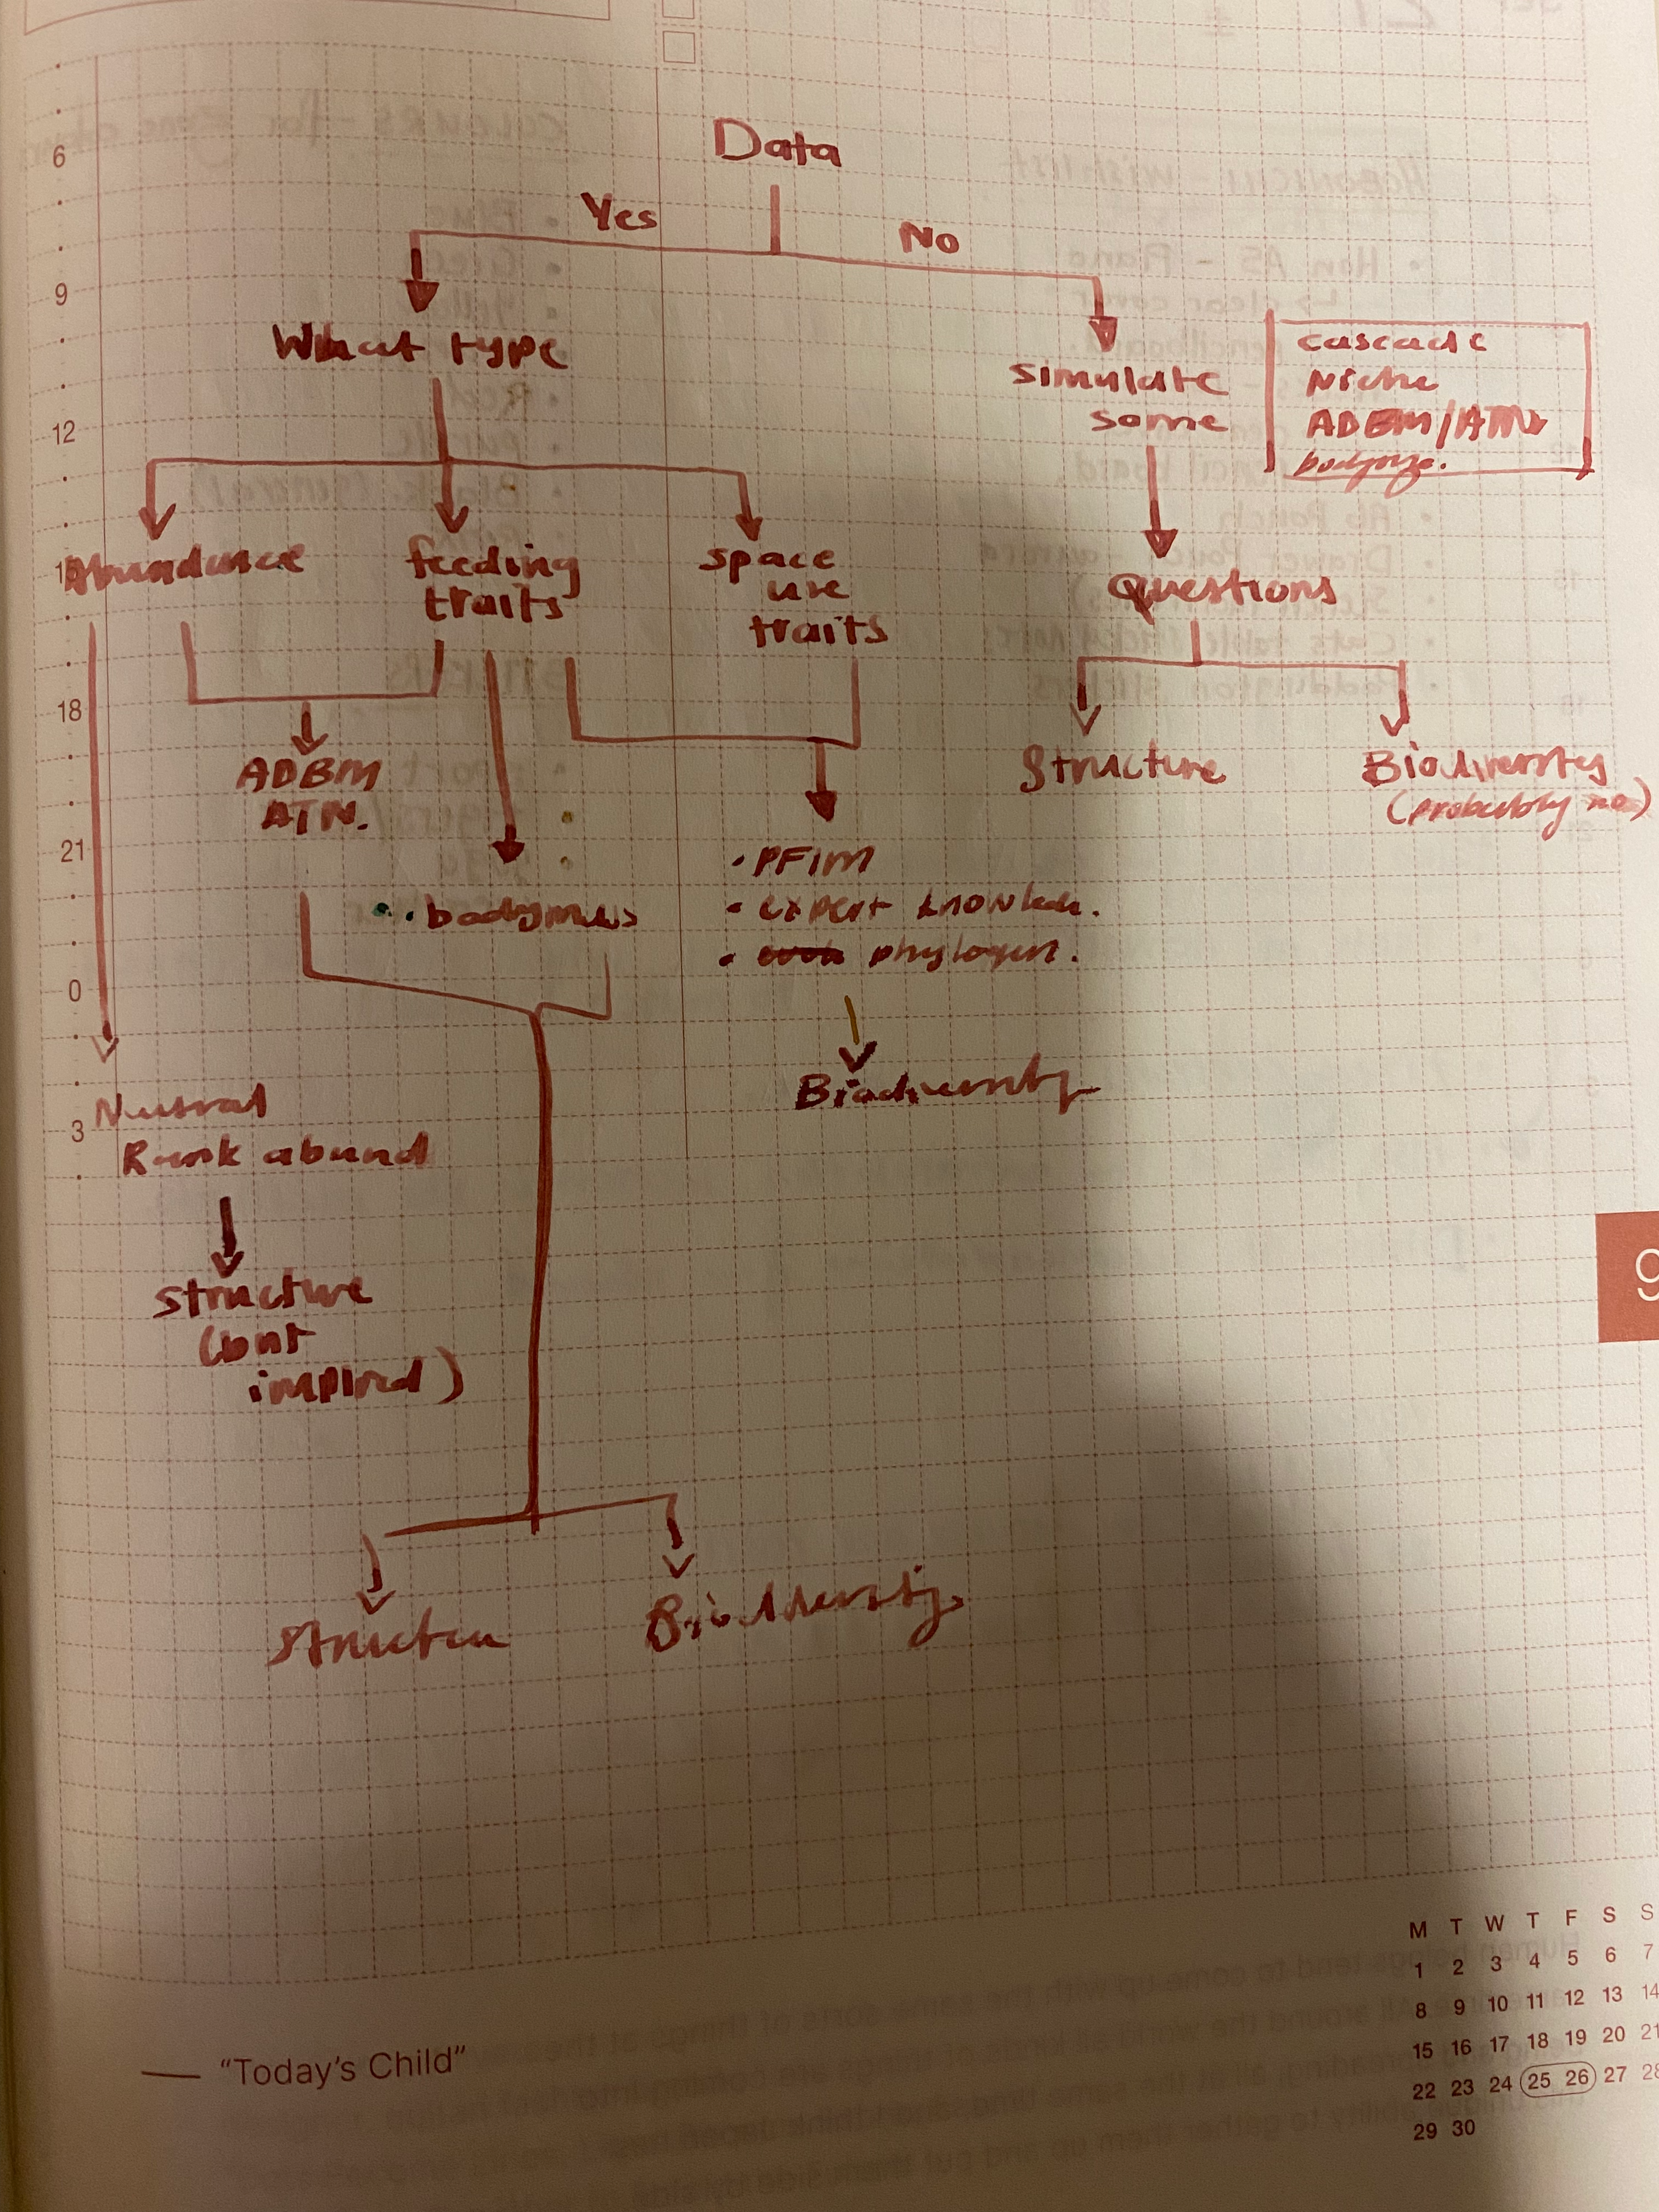
\includegraphics[keepaspectratio]{figures/guidelines.png}}

}

\caption{\label{fig-guidelines}TODO.}

\end{figure}%

\section*{References}\label{references}
\addcontentsline{toc}{section}{References}

\phantomsection\label{refs}
\begin{CSLReferences}{1}{0}
\bibitem[\citeproctext]{ref-allesina2008}
Allesina, S., Alonso, D., \& Pascual, M. (2008). A general model for
food web structure. \emph{Science}, \emph{320}(5876), 658--661.
\url{https://doi.org/10.1126/science.1156269}

\bibitem[\citeproctext]{ref-bambach2007}
Bambach, R. K., Bush, A. M., \& Erwin, D. H. (2007). Autecology and the
Filling of Ecospace: Key Metazoan Radiations. \emph{Palaeontology},
\emph{50}(1), 1--22.
\url{https://doi.org/10.1111/j.1475-4983.2006.00611.x}

\bibitem[\citeproctext]{ref-delmas2018}
Delmas, E., Besson, M., Brice, M.-H., Burkle, L. A., Dalla Riva, G. V.,
Fortin, M.-J., Gravel, D., Guimarães, P. R., Hembry, D. H., Newman, E.
A., Olesen, J. M., Pires, M. M., Yeakel, J. D., \& Poisot, T. (2018).
Analysing ecological networks of species interactions. \emph{Biological
Reviews}, 112540. \url{https://doi.org/10.1111/brv.12433}

\bibitem[\citeproctext]{ref-dillon2022}
Dillon, E. M., Pier, J. Q., Smith, J. A., Raja, N. B., Dimitrijević, D.,
Austin, E. L., Cybulski, J. D., De Entrambasaguas, J., Durham, S. R.,
Grether, C. M., Haldar, H. S., Kocáková, K., Lin, C.-H., Mazzini, I.,
Mychajliw, A. M., Ollendorf, A. L., Pimiento, C., Regalado Fernández, O.
R., Smith, I. E., \& Dietl, G. P. (2022). What is conservation
paleobiology? Tracking 20 years of research and development.
\emph{Frontiers in Ecology and Evolution}, \emph{10}.
\url{https://doi.org/10.3389/fevo.2022.1031483}

\bibitem[\citeproctext]{ref-dunhill2024}
Dunhill, A. M., Zarzyczny, K., Shaw, J. O., Atkinson, J. W., Little, C.
T. S., \& Beckerman, A. P. (2024). Extinction cascades, community
collapse, and recovery across a Mesozoic hyperthermal event.
\emph{Nature Communications}, \emph{15}(1), 8599.
\url{https://doi.org/10.1038/s41467-024-53000-2}

\bibitem[\citeproctext]{ref-dunne2014}
Dunne, J. A., Labandeira, C. C., \& Williams, R. J. (2014). Highly
resolved early eocene food webs show development of modern trophic
structure after the end-cretaceous extinction. \emph{Proceedings of the
Royal Society B: Biological Sciences}, \emph{281}(1782), 20133280.
\url{https://doi.org/10.1098/rspb.2013.3280}

\bibitem[\citeproctext]{ref-dunne2008}
Dunne, J. A., Williams, R. J., Martinez, N. D., Wood, R. A., \& Erwin,
D. H. (2008). Compilation and Network Analyses of Cambrian Food Webs.
\emph{PLOS Biology}, \emph{6}(4), e102.
\url{https://doi.org/10.1371/journal.pbio.0060102}

\bibitem[\citeproctext]{ref-erdos1959}
Erdős, P., \& Rényi, A. (1959). On random graphs. i. \emph{Publicationes
Mathematicae Debrecen}, \emph{6}(3-4), 290--297.
\url{https://doi.org/10.5486/pmd.1959.6.3-4.12}

\bibitem[\citeproctext]{ref-fricke2022}
Fricke, E. C., Hsieh, C., Middleton, O., Gorczynski, D., Cappello, C.
D., Sanisidro, O., Rowan, J., Svenning, J.-C., \& Beaudrot, L. (2022).
Collapse of terrestrial mammal food webs since the Late Pleistocene.
\emph{Science}, \emph{377}(6609), 1008--1011.
\url{https://doi.org/10.1126/science.abn4012}

\bibitem[\citeproctext]{ref-gupta2022}
Gupta, A., Furrer, R., \& Petchey, O. L. (2022). Simultaneously
estimating food web connectance and structure with uncertainty.
\emph{Ecology and Evolution}, \emph{12}(3), e8643.
\url{https://doi.org/10.1002/ece3.8643}

\bibitem[\citeproctext]{ref-hao2025}
Hao, X., Holyoak, M., Zhang, Z., \& Yan, C. (2025). Global Projection of
Terrestrial Vertebrate Food Webs Under Future Climate and Land-Use
Changes. \emph{Global Change Biology}, \emph{31}(2), e70061.
\url{https://doi.org/10.1111/gcb.70061}

\bibitem[\citeproctext]{ref-ings2009}
Ings, T. C., Montoya, J. M., Bascompte, J., Blüthgen, N., Brown, L.,
Dormann, C. F., Edwards, F., Figueroa, D., Jacob, U., Jones, J. I.,
Lauridsen, R. B., Ledger, M. E., Lewis, H. M., Olesen, J. M., Veen, F.
J. F. van, Warren, P. H., \& Woodward, G. (2009). Ecological
networks--beyond food webs. \emph{The Journal of Animal Ecology},
\emph{78}(1), 253--269.
\url{https://doi.org/10.1111/j.1365-2656.2008.01460.x}

\bibitem[\citeproctext]{ref-jenny2019}
Jenny, D., Fuchs, D., Arkhipkin, A. I., Hauff, R. B., Fritschi, B., \&
Klug, C. (2019). Predatory behaviour and taphonomy of a Jurassic
belemnoid coleoid (Diplobelida, Cephalopoda). \emph{Scientific Reports},
\emph{9}(1), 7944. \url{https://doi.org/10.1038/s41598-019-44260-w}

\bibitem[\citeproctext]{ref-jordano2016}
Jordano, P. (2016). Sampling networks of ecological interactions.
\emph{Functional Ecology}, \emph{30}(12), 1883--1893.
\url{https://doi.org/10.1111/1365-2435.12763}

\bibitem[\citeproctext]{ref-kiessling2019}
Kiessling, W., Raja, N. B., Roden, V. J., Turvey, S. T., \& Saupe, E. E.
(2019). Addressing priority questions of conservation science with
palaeontological data. \emph{Philosophical Transactions of the Royal
Society B: Biological Sciences}, \emph{374}(1788), 20190222.
\url{https://doi.org/10.1098/rstb.2019.0222}

\bibitem[\citeproctext]{ref-milo2002}
Milo, R., Shen-Orr, S., Itzkovitz, S., Kashtan, N., Chklovskii, D., \&
Alon, U. (2002). Network motifs: Simple building blocks of complex
networks. \emph{Science}, \emph{298}(5594), 824--827.
\url{https://doi.org/10.1126/science.298.5594.824}

\bibitem[\citeproctext]{ref-morales-castilla2015}
Morales-Castilla, I., Matias, M. G., Gravel, D., \& Araújo, M. B.
(2015). Inferring biotic interactions from proxies. \emph{Trends in
Ecology \& Evolution}, \emph{30}(6), 347--356.
\url{https://doi.org/10.1016/j.tree.2015.03.014}

\bibitem[\citeproctext]{ref-petchey2008}
Petchey, O. L., Beckerman, A. P., Riede, J. O., \& Warren, P. H. (2008).
Size, foraging, and food web structure. \emph{Proceedings of the
National Academy of Sciences}, \emph{105}(11), 4191--4196.
\url{https://doi.org/10.1073/pnas.0710672105}

\bibitem[\citeproctext]{ref-pichler2023}
Pichler, M., \& Hartig, F. (2023). Machine learning and deep
learning{\textemdash}A review for ecologists. \emph{Methods in Ecology
and Evolution}, \emph{14}(4), 994--1016.
\url{https://doi.org/10.1111/2041-210X.14061}

\bibitem[\citeproctext]{ref-poisot2012}
Poisot, T., Canard, E., Mouquet, N., \& Hochberg, M. E. (2012). A
comparative study of ecological specialization estimators. \emph{Methods
in Ecology and Evolution}, \emph{3}(3), 537--544.
\url{https://doi.org/10.1111/j.2041-210x.2011.00174.x}

\bibitem[\citeproctext]{ref-rohr2010}
Rohr, R., Scherer, H., Kehrli, P., Mazza, C., \& Bersier, L.-F. (2010).
Modeling food webs: Exploring unexplained structure using latent traits.
\emph{The American Naturalist}, \emph{176}(2), 170--177.
\url{https://doi.org/10.1086/653667}

\bibitem[\citeproctext]{ref-roopnarine2006}
Roopnarine, P. D. (2006). Extinction cascades and catastrophe in ancient
food webs. \emph{Paleobiology}, \emph{32}(1), 1--19.
\url{https://www.jstor.org/stable/4096814}

\bibitem[\citeproctext]{ref-schneider2016}
Schneider, F. D., Brose, U., Rall, B. C., \& Guill, C. (2016). Animal
diversity and ecosystem functioning in dynamic food webs. \emph{Nature
Communications}, \emph{7}(1), 12718.
\url{https://doi.org/10.1038/ncomms12718}

\bibitem[\citeproctext]{ref-shaw2024}
Shaw, J. O., Dunhill, A. M., Beckerman, A. P., Dunne, J. A., \& Hull, P.
M. (2024). \emph{A framework for reconstructing ancient food webs using
functional trait data} (p. 2024.01.30.578036). bioRxiv.
\url{https://doi.org/10.1101/2024.01.30.578036}

\bibitem[\citeproctext]{ref-stouffer2007}
Stouffer, D. B., Camacho, J., Jiang, W., \& Nunes Amaral, L. A. (2007).
Evidence for the existence of a robust pattern of prey selection in food
webs. \emph{Proceedings of the Royal Society B: Biological Sciences},
\emph{274}(1621), 1931--1940.
\url{https://doi.org/10.1098/rspb.2007.0571}

\bibitem[\citeproctext]{ref-strydom2021}
Strydom, T., Catchen, M. D., Banville, F., Caron, D., Dansereau, G.,
Desjardins-Proulx, P., Forero-Muñoz, N. R., Higino, G., Mercier, B.,
Gonzalez, A., Gravel, D., Pollock, L., \& Poisot, T. (2021). A roadmap
towards predicting species interaction networks (across space and time).
\emph{Philosophical Transactions of the Royal Society B: Biological
Sciences}, \emph{376}(1837), 20210063.
\url{https://doi.org/10.1098/rstb.2021.0063}

\bibitem[\citeproctext]{ref-thuiller2024}
Thuiller, W., Calderón-Sanou, I., Chalmandrier, L., Gaüzère, P.,
O'Connor, L. M. J., Ohlmann, M., Poggiato, G., \& Münkemüller, T.
(2024). Navigating the integration of biotic interactions in
biogeography. \emph{Journal of Biogeography}, \emph{51}(4), 550--559.
\url{https://doi.org/10.1111/jbi.14734}

\bibitem[\citeproctext]{ref-vullo2011}
Vullo, R. (2011). Direct evidence of hybodont shark predation on Late
Jurassic ammonites. \emph{Naturwissenschaften}, \emph{98}(6), 545--549.
\url{https://doi.org/10.1007/s00114-011-0789-9}

\bibitem[\citeproctext]{ref-williams2000}
Williams, R. J., \& Martinez, N. D. (2000). Simple rules yield complex
food webs. \emph{Nature}, \emph{404}(6774), 180--183.
\url{https://doi.org/10.1038/35004572}

\bibitem[\citeproctext]{ref-williams2004}
Williams, R. J., \& Martinez, N. D. (2004). Stabilization of chaotic and
non-permanent food-web dynamics. \emph{The European Physical Journal B -
Condensed Matter}, \emph{38}(2), 297--303.
\url{https://doi.org/10.1140/epjb/e2004-00122-1}

\bibitem[\citeproctext]{ref-williams2008}
Williams, R. J., \& Martinez, N. D. (2008). Success and its limits among
structural models of complex food webs. \emph{The Journal of Animal
Ecology}, \emph{77}(3), 512--519.
\url{https://doi.org/10.1111/j.1365-2656.2008.01362.x}

\bibitem[\citeproctext]{ref-yeakel2014}
Yeakel, J. D., Pires, M. M., Rudolf, L., Dominy, N. J., Koch, P. L.,
Guimarães, P. R., \& Gross, T. (2014). Collapse of an ecological network
in ancient egypt. \emph{PNAS}, \emph{111}(40), 14472--14477.
\url{https://doi.org/10.1073/pnas.1408471111}

\end{CSLReferences}





\end{document}
